\documentclass[conference]{IEEEtran}
\IEEEoverridecommandlockouts

% Preserve the original Times/Helvetica typography across TeX engines.
\usepackage[T1]{fontenc}
\usepackage{times}
\usepackage{graphicx}
\usepackage{url}

\usepackage{tikz}
\usetikzlibrary{arrows.meta,positioning,shapes.multipart,fit,calc}
\usepackage[hidelinks]{hyperref}
\hypersetup{
  pdftitle={Protein Discovery for Pollution Mitigation},
  pdfauthor={Santiago Restrepo},
  pdfsubject={Waajacu research project - Cleaning the Brahmaputra},
  pdfkeywords={Waajacu, Brahmaputra, bioremediation, protein screening}
}

\begin{document}

\title{Protein Discovery for Pollution Mitigation}

\author{\IEEEauthorblockN{Santiago Restrepo}
\IEEEauthorblockA{\textbf{Waajacu}\\
\url{https://waajacu.com/}}
}


\IEEEaftertitletext{%
  \noindent\begin{minipage}{\textwidth}
  \centering
  \resizebox{\textwidth}{!}{%


\begin{tikzpicture}[
  font=\sffamily,
  node distance=10mm and 22mm,
  >=Latex,
  line/.style={-Latex, very thick},
  box/.style={
    rounded corners=7pt, inner sep=7pt, minimum height=13mm,
    draw=black, thick, align=center
  },
  % palette
  saffron/.style={fill={rgb,255:red,255;green,214;blue,163}},
  CandidateI/.style={fill={rgb,255:red,240;green,223;blue,255}},
  grayI/.style={fill={rgb,255:red,242;green,242;blue,242}}
]

% --- INPUT (left) ---
\node[box,saffron,text width=48mm,align=center,inner sep=8pt] (poll) {%
    \textbf{Fix a Pollutant}\\
    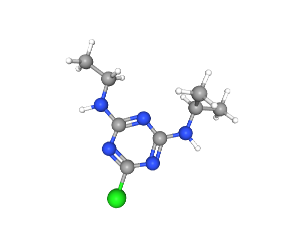
\includegraphics[width=48mm]{atrazine.png}\\[-1mm]
    \footnotesize Atrazine (PubChem CID 2256)
};

% --- SEARCH STACK (center) ---
\node[box,grayI,right=30mm of poll,text width=73mm,align=left] (gnina) {%
\textbf{AI Catalytic Scoring (GNINA)}\\[4mm]
\footnotesize Vina-style pose search with ensemble CNN rescoring.\\
\footnotesize \textit{Inputs:} ligand = pollutant (fixed); receptor = protein.\\
\footnotesize Used as a screening proxy (not catalytic proof).%
};


\node[box,CandidateI,below=16mm of gnina,text width=62mm,align=center,inner sep=8pt] (prot) {%
    \textbf{Candidate Proteins}\\
    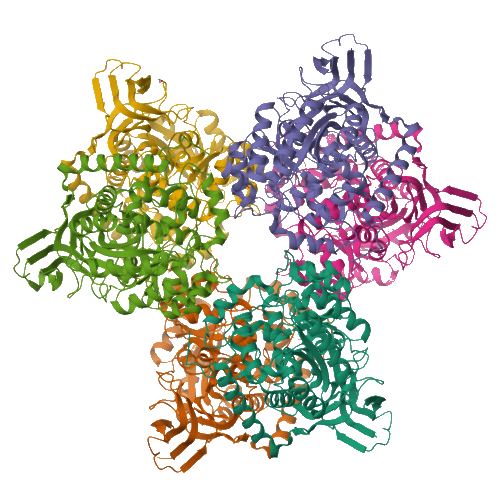
\includegraphics[width=48mm]{4v1y.png}\\[-0.5mm]
    \footnotesize AtzA (Pseudomonas sp. ADP) \textemdash{} PDB 4V1Y
};

% Search group box with title
\node[
  draw, rounded corners=10pt, thick,
  fit={(gnina) (prot)},
  inner sep=10pt,
  label={[font=\small\bfseries]above:Search}
] (searchbox) {};

% --- OUTPUT (right) ---
\node[box,saffron,right=28mm of searchbox,text width=60mm,align=left] (out) {%
\textbf{Output: Top-$k$ Enzymes}\\[1mm]
\footnotesize for the selected pollutant\\[1mm]
\footnotesize 1.\ \texttt{PDB: XXXX} (\(-7.8\))\\
\footnotesize 2.\ \texttt{PDB: YYYY} (\(-7.2\))\\
\footnotesize 3.\ \texttt{PDB: ZZZZ} (\(-6.9\))\\
\footnotesize \dots
};

% --- EXTERNAL FLOW: arrows touch the Search box, not GNINA ---
\draw[line] (poll.east) -- node[midway,above]{} (gnina.west);
\draw[line] (searchbox.east) -- node[midway,above]{} (out.west);

% --- INTERNAL LOOP (clean vertical, no rotated text) ---
% down: GNINA -> PROT (left side)
\draw[line] ([xshift=-12mm]gnina.south) to[out=-90,in=90]
  node[midway,left,font=\footnotesize]{}
  ([xshift=-12mm]prot.north);
% up: PROT -> GNINA (right side)
\draw[line] ([xshift=12mm]prot.north) to[out=90,in=-90]
  node[midway,right,font=\footnotesize]{random batch}
  ([xshift=12mm]gnina.south);

% Optional column captions
\node[font=\footnotesize] at ($(out)+(0,18mm)$) {Result};
\end{tikzpicture}


  }
  \par\smallskip
  \small\textbf{Figure 1.} Pollutant-Enzyme exploration workflow diagram.
  \end{minipage}\par\medskip
}

\maketitle

\begin{abstract}
    This work presents a demonstration of how open-source tools and freely available databases can be integrated to explore possible 
    bioremediation strategies. No new algorithms or methods are introduced. Instead, we show how existing resources can be combined 
    into a workflow that identifies candidate protein structures with potential to interact with common pollutants. The demonstration 
    focuses on pollutants reported in the Brahmaputra.
\end{abstract}

\section{Introduction}
Industrial and agricultural waste contribute significantly to water pollution in major river systems such as the Brahmaputra. 
While global research in protein engineering and biocatalysis continues to advance, the goal of this Waajacu project is not to propose 
novel science. Rather, we illustrate how openly available computational tools and datasets can be chained together 
to demonstrate a possible pathway toward protein-based pollution mitigation.



\section{Methodology}

\textbf{Inputs.}
\emph{Pollutants} (SDF; \url{https://pubchem.ncbi.nlm.nih.gov}) and \emph{candidate receptor proteins}
(PDB; \url{https://www.rcsb.org}). For the demo, we \emph{fix one pollutant} as the ligand and explore a pool
of proteins via random sampling.

\textbf{Search strategy.}
With the pollutant held fixed, we iterate over batches of proteins from PDB. 
Each batch is evaluated and the current top-$k$ is updated.

\textbf{Docking \& AI scoring (GNINA).}
Protein-pollutant interaction is estimated with GNINA
(\url{https://github.com/gnina/gnina}), using a Vina-style pose search with
ensemble CNN re-scoring. The primary readout is predicted binding affinity (kcal/mol),
where \emph{more negative is better}. 

\textbf{Selection \& output.}
Receptors are ranked by their best-pose affinity. The deliverable is the
\emph{ranked top-$k$ enzymes} (PDB IDs with predicted affinities) for the fixed pollutant.
Scores are used strictly as a \emph{screening proxy} for interaction strength and do not
establish catalytic viability; experimental validation is required. 

\section{Conclusion}
This Waajacu project explores protein-based pollution mitigation.
It shows how open-source AI tools and public databases can be chained into a transparent, 
reproducible screening workflow. Framed around the Brahmaputra pollution context,
it highlights how existing resources can help identify candidate enzymes for further research.

\begin{thebibliography}{00}

\bibitem{rcsb}
RCSB Protein Data Bank (RCSB PDB). Accessed: Aug. 18, 2025. [Online]. \url{https://www.rcsb.org}
\bibitem{pubchem}
National Center for Biotechnology Information (NCBI), PubChem. Accessed: Aug. 18, 2025. [Online]. \url{https://pubchem.ncbi.nlm.nih.gov}
\bibitem{gnina}
Gnina: Deep Learning Framework for Molecular Docking (GitHub). Accessed: Aug. 18, 2025. [Online]. \url{https://github.com/gnina/gnina}
\end{thebibliography}

\end{document}
